\documentclass[12pt]{report}
\usepackage[utf8x]{inputenc}
\usepackage[serbianc]{babel}
\usepackage{subcaption}
\usepackage {graphicx}
\usepackage{float}
\usepackage{gensymb}
\def\figurename{slika}
\def\tablename{табела}
\usepackage[section]{placeins}
\usepackage{makecell}
\usepackage{amsmath}
\usepackage[a4paper, total={6.5in, 9.4in}]{geometry}
\newtheorem{theorem}{\bf Теорема}[section]
\newtheorem{lemma}[theorem]{\bf Лема}
\newtheorem{corollary}[theorem]{\bf Последица}
\newtheorem{definition}[theorem]{\bf Дефиниција}
\newtheorem{conjecture}[theorem]{\bf Хипотеза}
\newtheorem{remark}[theorem]{\bf Примедба}
\newtheorem{problem}[theorem]{\bf Проблем}
\newtheorem{alg}[theorem]{\bf Алгоритам}
\newtheorem{pri}{\bf Пример}
\newtheorem{tvrdjenje}{\bf Тврђење}

\newcommand{\comment}[1]{\ $[\![${\normalsize #1}$]\!]$ \ }
\newcommand{\proof}{\noindent{\bf Доказ\ }}
\newcommand{\qed}{\hfill $\square$ \bigskip}
\def\cp{\,\square\,}



\usepackage[colorlinks = false,
            linkcolor = blue,
            urlcolor  = blue,
            citecolor = blue,
            anchorcolor = blue]{hyperref}


\begin{document}


\newcommand{\HRule}{\rule{\linewidth}{0.5mm}} % Defines a new command for the horizontal lines, change thickness here

\thispagestyle{empty}
\\
\centerline{\LARGE \textbf{МАТЕМАТИЧКА ГИМНАЗИЈА}}

\vspace*{40mm}
\begin{center}
{\Large МАТУРСКИ РАД}\\
{\Large	из предмета}\\
{\Large	aнализа са алгебром}\\
{\Large	на тему}
\Huge\HRule\\[0.4cm] %0.4cm
	{Конструисање поплочавања еуклидске равни}\\
	\HRule \\[20pt] %20pt
\begin{minipage}{0.4\textwidth}
\begin{flushleft} \large
\emph{\Large Ученик:}\\
{\Large Марина Васиљевић}, IV$_\text{Е}$\\
\end{flushleft}
\end{minipage}
~
\begin{minipage}{0.4\textwidth}
\begin{flushright} \large
\vspace{0.5cm}
\emph{\Large Ментор:} \\
{\Large Зоран Лучић}\\ 
\end{flushright}
\end{minipage}\\[8cm]
\Large{Београд, мај 2019.}
\end{center}

\tableofcontents

\thispagestyle{empty}

\clearpage
\setcounter{page}{1}

\chapter{Увод}
Људи су одувек имали потребу за украшавањем простора у којем бораве.  Откада је човек почео да користи камен за облагање зидова и подова, почео је и да бира камење по боји и облику и на тај начин прави шаре.
У свим земљама могу се наћи површи прекривене облицима који се слажу и стварају неку шару. Понављање неких облика доста је заступљено у орнаменталној уметности и мозаику.
Стари Грци и Римљани правили су мозаике који су приказивали сцене из историје, митологије или свакодневног живота. (слика 1). Са друге стране, Арапи и Маври користили су плочице у само неколико боја и облика и на тај начин правили занимљиве шаре којима су украшавали своје грађевине. Један такав пример је палата Алхамбра у Шпанији (слика 2). Данас се за поплочавања обично користе једноставни облици али се уметници као што је Морис Ешер \footnote{Maurits Cornelis Escher - холандски уметник и графичар, посебно познат по својим представама парадоксалних и немогућих призора (1898—1972)} баве занимљивим понављајућим шарама, као видом уметности (слика 3).
Иако сe дизајнирањем поплочавања људи баве хиљадама година, тек крајем 19. века настају први помаци у њиховом математичком објашњењу. (ВАЉДА?)

У раду се бавимо математичким представљањем поплочавања као и имлпементацијом интерактивне апликације којом се према инструкцијама корисника могу добити поплочавања.





\chapter{Увод у поплочавања}\label{kristalografske-grupe-i-poploux10davanje}
%\section{Математичко представљање поплочавања}
Поплочавање је прекривање равни или простора геометријским фигурама чије се унутрашњости не преклапају. Такве фигуре називамо плочицама или теселима од латинске речи \emph{tessalla} која означава парче камена или стакла од кога се слаже мозаик. Посебно
су занимљива поплочавања код којих су плочице подударне, односно за сваке две плочице постоји пресликавање које чува растојања између тачака, односно \emph{изометријска трансформација}. Такво поплочавање назива се \emph{моноедарско}.

У овом раду ћемо се бавити поплочавањима еуклидске равни
\(\mathbb{E}^2\). Прво ћемо дефинисати појам изометријске трансформације.

\begin{definition}
Бијекција $\sigma \! : \, \mathbb{E}^2 \xrightarrow \mathbb{E}^2$ је изометријска трансформација ако сваке две тачке $A, B$ пресликава у $A',B'$ такo да је $AB \cong A'B'$.
\end{definition}

Све изометрије равни су једног од четири типа:
\begin{enumerate}
    \item Транслација за дати вектор $v$, у ознаци $\mathcal{T}_v$(слика)
    \item Ротација око тачке $O$ зa угао $\varphi$, у ознаци $\mathcal{R}_{O,\varphi}$. Специјално, када је $\varphi = \pi$ назива се \emph{централна симетрија} у тачки $O$ и означава само $\mathcal{R}_O$
    \item Рефлексија са осом $p$, у ознаци $\mathcal{S}_p$ (слика)
    \item Клизајућа рефлексија, односно композиција рефлексије са осом $p$ и транслације за вектор $v$, колинеаран са осом, означава се са $\mathcal{G}_{v,p}$ (слика)
\end{enumerate} 

\begin{figure}[H]

  \begin{subfigure}[b]{0.22\textwidth}
    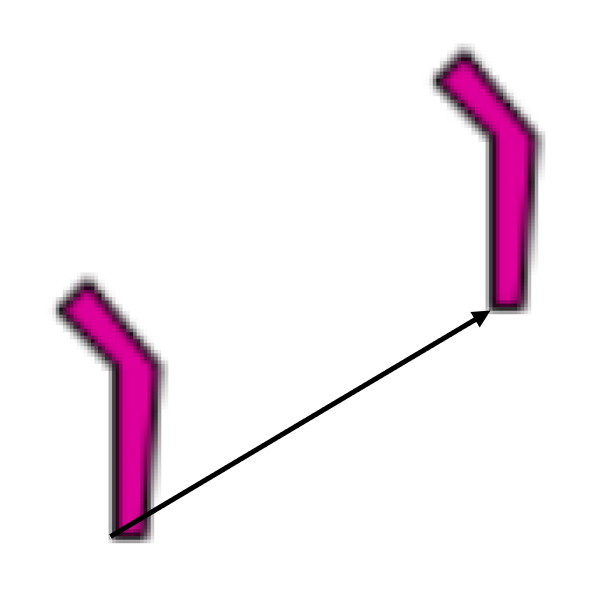
\includegraphics[width=.9\textwidth]{crtez_translacija.png}
    \label{fig:f4}
    %\caption{Транслација}

  \end{subfigure}
  \begin{subfigure}[b]{0.24\textwidth}
    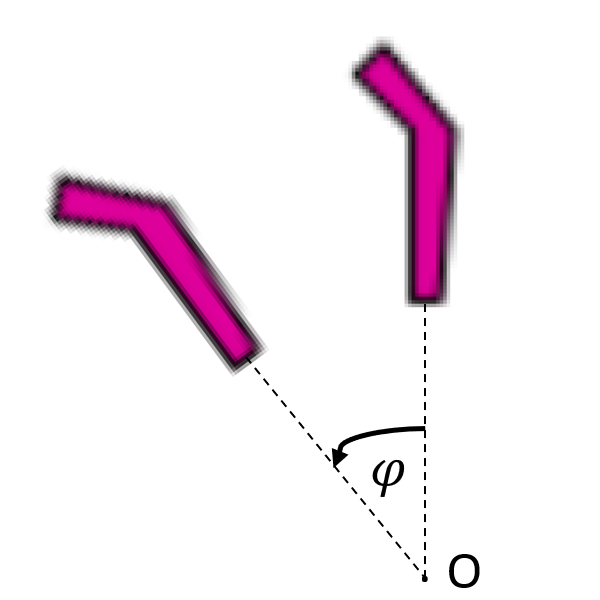
\includegraphics[width=.9\textwidth]{crtez_rotacija.png}
    \label{fig:f5}
    %\caption{Ротација}
    \end{subfigure}
  \begin{subfigure}[b]{0.24\textwidth}
    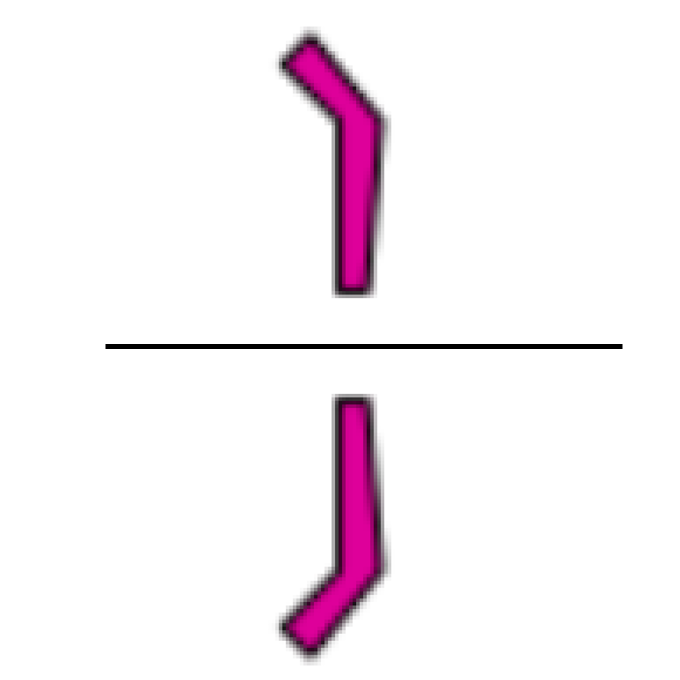
\includegraphics[width=.9\textwidth]{crtez_refleksija.png}
    %\caption{Рефлексија}
    \label{fig:f5}
    
\end{subfigure}
\begin{subfigure}[b]{0.24\textwidth}
    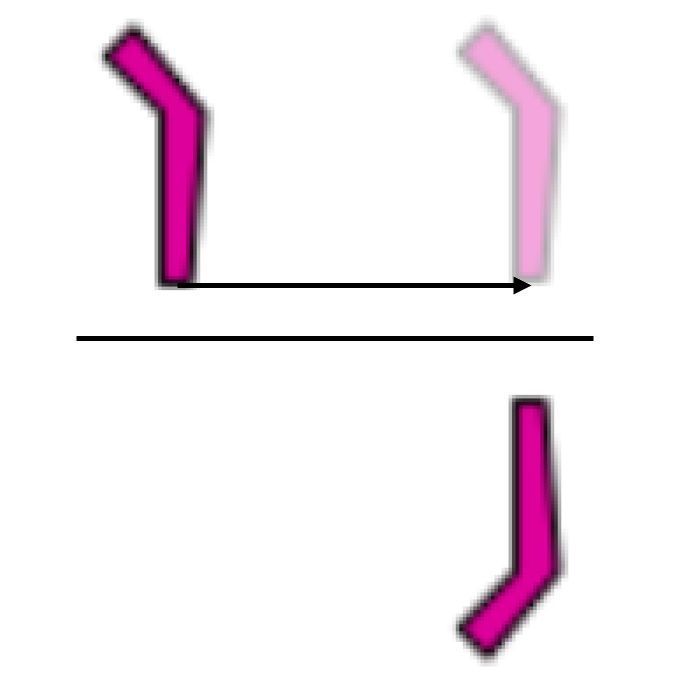
\includegraphics[width=.9\textwidth]{crtez_klizajuca.png}
    %\caption{Клизајућа}
    \label{fig:f5}
    
\end{subfigure}
\caption{Изометријске трансформације}
\end{figure}


Изометрија је \emph{директна} ако задржава оријентацију, односно ако се сваки троугао равни слика у троугао који је исто оријентисан (слика). Директне изометрије су транслација и ротација. Рефлексија и клизајућа рефлексија су \emph{индиректне} што значи да се сваки троугао слика у троугао супротне оријентације (слика

Изометрија која сваку тачку слика у саму себе назива се \emph{идентитет} и означава са $\mathcal{I}$.

Скуп свих изометрија са операцијом композиције је алгебарска структура група јер
\begin{enumerate}
    \item Композиција идентитета и било које изометрије даје ту изометрију
    
    \item Свака изометрија има себи инверзну изометрију:
    \begin{itemize}
        \item $\mathcal{T}_v \circ \mathcal{T}_{-v} = \mathcal{I}$
        \item $\mathcal{R}_{O,\varphi} \circ \mathcal{R}_{O,-\varphi} = \mathcal{I}$
        \item $\mathcal{S}_p \circ \mathcal{S}_p = \mathcal{I}$
        \item $\mathcal{G}_{v,p} \circ \mathcal{G}_{-v,p} = \mathcal{I}$
    \end{itemize}
    \item Композиција две изометрије је такође изометријa.
\end{enumerate}
Сваку подргрупу те групе називамо \emph{групом изометрија}. 

Симетрија неке фигуре $T$ је изометрија $\sigma$ таква да слика $Т$ у саму себе односно $\sigma T = T$. Скуп свих симетрија једне фигуре је подгрупа групе свих симетрија равни зато што
\begin{enumerate}
    \item Идентитет је симетрија сваке фигуре
    \item Инверз симетрије неке фигуре је такође симетрија те фигуре
    \item Композиција две симетрије исте фигуре је симетрија те фигуре.
\end{enumerate}

Зато скуп свих симетрија једне фигуре називамо \emph{групом симетрија} те фигуре.
\newline



Симетрије квадрата приказаног на слици 2.2 су рефлексије са осама $p_1,\, p_2,\, p_3$ i $p_4$, ротације око тачке $O$ за углове $90\degree,\, 180\degree$ и $ 270\degree$, као и идентитет.
 
 
 
\begin{figure}[H]
\centering
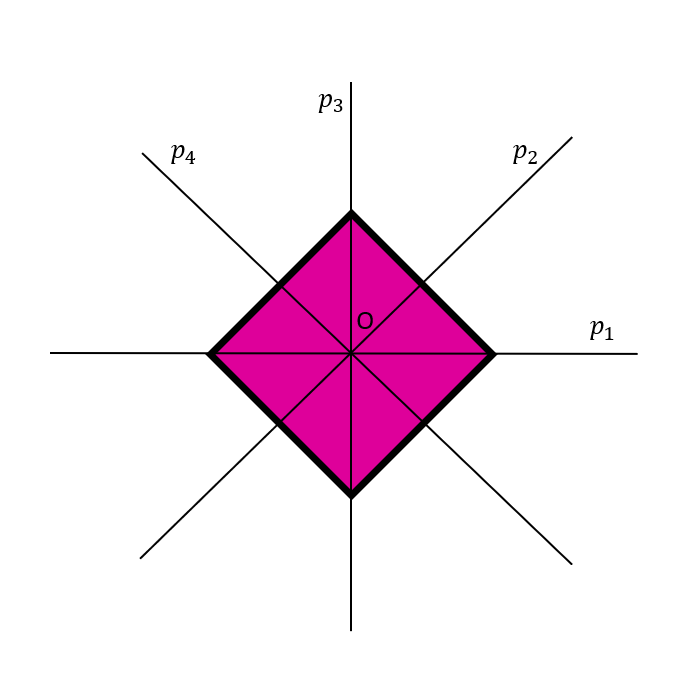
\includegraphics[width=0.45\textwidth]{Simetrije_kocke.png}
\caption{Симетрије квадрата}

\end{figure}





Симетрија поплочавања $\tau$ је изометрија која сваку плочицу тог пресликавања пресликава на неку другу плочицу.*стићи ће пример некад*
Ако група симетрија поплочавања садржи две неколинеарне транслације тада је поплочавање \emph{периодично}. То значи да група симетрија периодичног поплочавања садржи подгрупу транслација. Означимо са $a$ и $b$ векторе транслација из генератора те подгрупе. Тада ту подгрупу чине све транслације за  векторе облика $na + mb$, где $n,m \in \mathbb{Z} $. Применом изометрија те подгрупе транслација на произвољну тачку добијју се темена решетке са паралелним ивицама. Добијене решетке подсећају на кристалне решетке па се такве групе називају \emph{кристалографске групе}.

\begin{definition}Kристалографска група је коначно генерисана група изометрија равни $\mathbb{E}^2$ која садржи неколинеарне транслације.
\end{definition}

Постоје и поплочавања која нису периодична, односно које немају симетрије које су неколинеарни вектори. На сликама се виде примери неких апериодичних поплочавања али се њима у даљњм раду нећемо бавити и под поплочавањем ћемо подразумевати периодично поплочавање. (слика)

На сликама ћемо изометрије представљати симболима који су дати у табели 1.
Познато је да над \(\mathbb{E}^2\) постоји 17 типова кристалографских група. Користећи симболе из табеле 1 описаћемо неке од тих група (слика коју имам).
    \begin{center}
\begin{tabular}{ r l }
 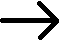
\includegraphics[width=.02\textwidth]{simbol7.png} & Транслација  \\ 
 
\includegraphics[width=.02\textwidth]{simbol2.png} & Ротација за угао 60\degree   \\  

\includegraphics[width=.02\textwidth]{simbol1.png} & Ротација за угао 60\degree   \\ 
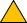
\includegraphics[width=.02\textwidth]{simbol4.png} & Ротација за угао 120\degree   \\ 

\includegraphics[width=.02\textwidth]{simbol3.png} & Централна симетрија   \\ 

\includegraphics[width=.02\textwidth]{simbol5.png} & Рефлексија  \\ 

\includegraphics[width=.02\textwidth]{simbol8.png} & Клизајућа рефлексија  
\end{tabular}
\caption{Симболи за представљање изометрија}
\end{center}

\begin{figure}[H]

  \begin{subfigure}[b]{0.32\textwidth}
    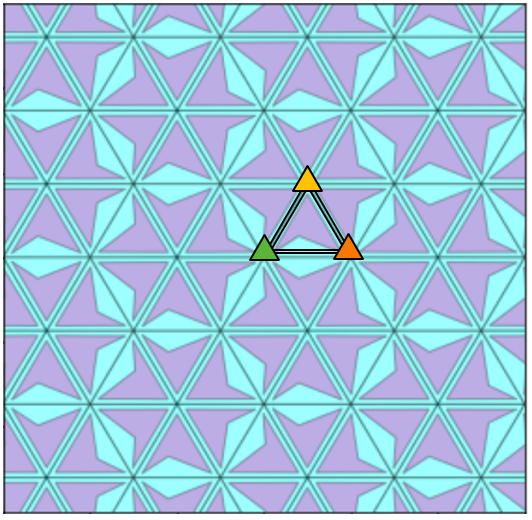
\includegraphics[width=.9\textwidth]{skicap3m1.png}
    \label{fig:f4}
  \end{subfigure}
  \begin{subfigure}[b]{0.32\textwidth}
    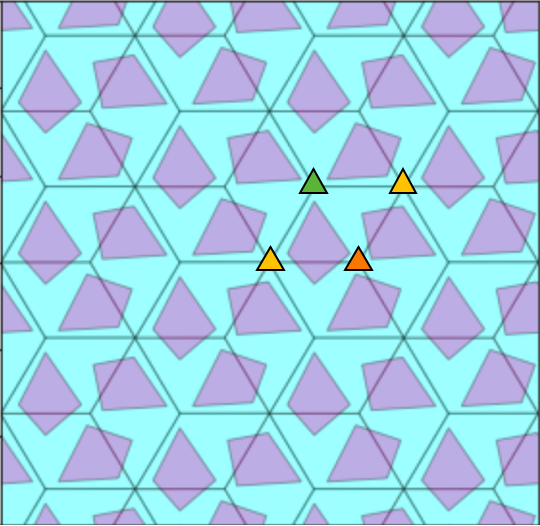
\includegraphics[width=.9\textwidth]{skicap3.png}
    \label{fig:f5}
    \end{subfigure}
  \begin{subfigure}[b]{0.32\textwidth}
    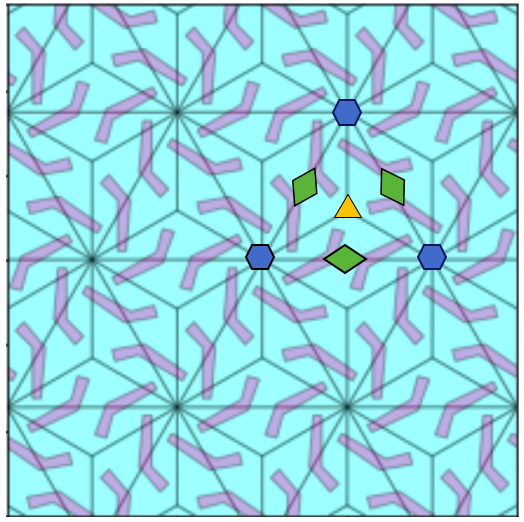
\includegraphics[width=.89\textwidth]{skicap6.png}
    \label{fig:f5}
    
\end{subfigure}
\caption{Примери кристалографских група приказаних симболима}

\end{figure}


Сва периодична поплочавања добијамо деловањем неке кристалографске групе на једну плочицу. Пример такве кристалографске групе је група симетрија поплочавања. Међутим, група која генерише поплочавање може бити права подгрупа групе симетрија уколико постоји нетривијална симетрија поплочавања која је уједино и симетрија плочице. У супротном, уколико ниједна нетривијална симетрија плочице није у групи која генерише поплочавање, та плочица је \emph{фундаментални домен} те групе.

\begin{definition} Фундаментални домен \(F\) кристалографске групе \(G\) равни \(\mathbb{E}^2\) је фигура таква да:\\
\begin{enumerate}
\item \(\displaystyle{\bigcup_{g\in G}g(F)} = \mathbb{E}^2\) 
\item \((\forall g\in G)(\mathring{F} \cap g(\mathring{F})= \emptyset)\) .
\end{enumerate}
\end{definition}

Поплочавање можемо конструисати тако што прво конструишемо кристалографску групу а затим њен фундаментални домен.Тиме ћемо се бавити у наставку рада као и рачунарском имплементацијом конструкције.

%група симетрија фигуре
%група симетрија поплочавања
%периодична попличавања
%фундаментална област групе
%кристалографкса група-кончнп генерисана и постоји полигална ф област

%тако да постоји група изометрија које једну фигуру пресликавају на све остале. Један од примера таквог поплочавања су кристалне решетке, због чега се такве групе називају кристалографским групама. 

%У оквиру овог рада бавићемо се својствима кристалографских група над \(\mathbb{E}^2\), својствима фундаменталних области и алгоритмима за конструисање фундаменталних полигона који на крају могу имати практичну примену у графичком дизајнирању поплочавања. Алгоритме ћемо имплементирати у програмском језику Пyтхон



    \chapter{\texorpdfstring{Конструкција кристалографских група
}{Izometrijske transformacije u \textbackslash{}mathbb\{Е\}\^{}2}}\label{izometrijske-transformacije-u-mathbbr2}
\section{Представљање изометрија аналитичком геометријом}

Да бисмо могли компјутерски да генеришемо поплочавање морамо прво конструисати кристалографску групу. Изометријске трансформације ћемо представити користећи аналитичку геометрију.

%За групу кажемо да је коначно генерисана ако постоји коначан подскуп елемената групе који генерише све елементе групе. У случају кристалографских група то је коначан скуп изометрија чијом композицијом добијамо све изометрије равни потребне за њено поплочавање датим фундаменталним доменом.

%\begin{definition} Кристалографска група је коначно
%генерисана периодична група изометрија.
%\end{definition}


    Ако у \(\mathbb{E}^2\) уведемо координатни систем, тачке представљамо
дводимензионим координатама тј. елементима \(\mathbb{R}^2\). Координате
тацке \(A\) означаваћемо са \((A_x, A_y)\). Аналитички ћемо изометријску
трансформацију у \(\mathbb{R}^2\) представити као специјалан случај
афине трансформације. Ако је \(A' = G(A)\) тада имамо:
\[A'_x = pA_x + qA_y + c_x\] \[A'_y = rA_x + sA_y + c_y\] 

Коришћењем
рачуна са матрицама то можемо представити:

\[\begin{bmatrix}p & q\\ r & s\end{bmatrix} \begin{bmatrix}A_x\\ A_y \end{bmatrix} + \begin{bmatrix}c_x\\ c_y\end{bmatrix} = \begin{bmatrix}A'_x\\ A'_y \end{bmatrix}\]

Претходна једнакост је еквивалентна следећој:

\[\begin{bmatrix}p & q & c_x\\ r & s&c_y \\ 0 & 0 & 1\end{bmatrix} \begin{bmatrix}A_x\\ A_y\\1\end{bmatrix} = 
\begin{bmatrix}A'_x\\ A'_y\\1\end{bmatrix}\]

Таква форма је погодна за рачунарску имплементацију јер се примена изометријске трансформације своди на  множење матрица. Посебно је значајно што се композиција изометријских трансформација своди на множење матрица одговарајућих изометрија. Заправо смо афине трансформације $\mathbb{R}^2$ представили као тродимензионе линеарне трансформације које $\mathbb{R}^2 \times \{ 1 \}$  сликају на исти тај скуп. Представљање тачака равни у $\mathbb{R}^2 \times \{ 1 \}$ назива се \emph{хомогеним координатама}.

На пример, матрица транслације $\mathcal{T}_t$ за вектор \( t = (t_x, t_y)\) је 

\[\begin{bmatrix}1 & 0 & t_x\\ 0 & 1&t_y \\ 0 & 0 & 1\end{bmatrix} \] 
јер
\[\begin{bmatrix}1 & 0 & t_x\\ 0 & 1&t_y \\ 0 & 0 & 1\end{bmatrix} \begin{bmatrix}A_x\\ A_y\\1\end{bmatrix} = 
\begin{bmatrix}A_x+t_x\\ A_y+t_y\\1\end{bmatrix}.\]



Једначина ротација за угао $\varphi$ око координатног почетка $\mathcal{R}_{O,\varphi}$ је $$A'_x = A_x  cos(\varphi) +  A_y  sin(\varphi)$$ 
$$A'_y = -A_x  sin(\varphi) + A_y  cos(\varphi)$$
што је у хомогеним координатама
\[\begin{bmatrix}cos(\varphi) & sin(\varphi) & 0\\ -sin(\varphi) & cos(\varphi)&0 \\ 0 & 0 & 1\end{bmatrix} \begin{bmatrix}A_x\\ A_y\\1\end{bmatrix} = 
\begin{bmatrix}A_x  cos(\varphi) +  A_y  sin(\varphi)\\ -A_x  sin(\varphi) + A_y  cos(\varphi)\\1\end{bmatrix}.\]

Једначина рефлексије око $x$-осе $\mathcal{S}_x$  у хомогеним координатама је
\[\begin{bmatrix}1 & 0 & 0\\ 0 & -1&0 \\ 0 & 0 & 1\end{bmatrix} \begin{bmatrix}A_x\\ A_y\\1\end{bmatrix} = 
\begin{bmatrix}A_x \\ -A_y\\1\end{bmatrix}.\]

Предност  коришћења  хомогених  координата  је  у  томе  што  слагање  изометрија  рачунамо  као множење матрица. Како ротацију око дате тачке $C$ можемо дефинисати као
$$\mathcal{R}_{C,\varphi} = \mathcal{T}_{\vec{OC}} \circ \mathcal{R}_{O,\varphi} \circ \mathcal{T}_{\vec{CO}}$$
што значи да матрицу ротације $\mathcal{R}_{C,\varphi}$ рачунамо као

\[\begin{bmatrix}1 & 0 & C_x\\ 0 & 1&C_y \\ 0 & 0 & 1\end{bmatrix}
\begin{bmatrix}cos(\varphi) & sin(\varphi) & 0\\ -sin(\varphi) & cos(\varphi)&0 \\ 0 & 0 & 1\end{bmatrix}
\begin{bmatrix}1 & 0 & -C_x\\ 0 & 1&-C_y \\ 0 & 0 & 1\end{bmatrix}
=  \]


\[\begin{bmatrix}cos(\varphi) & sin(\varphi) & -C_x cos(\varphi) - C_y sin(\varphi) + C_x\\ -sin(\varphi) & cos(\varphi)&C_x sin(\varphi) - C_y cos(\varphi) +y\\ 0 & 0 & 1\end{bmatrix}.\]

Слично конструишемо рефлексију око произвољне осе $p$ задате координатама тачке $A$ на њој и углом $\varphi$ који она гради са x-осом
$$\mathcal{S}_{p} = \mathcal{T}_{\vec{OA}} \circ \mathcal{R}_{O,\varphi} \circ \mathcal{S}_{x} \circ \mathcal{R}_{O,-\varphi} \circ \mathcal{T}_{\vec{AO}}.$$

Уколико оса пролази кроз координатни почетак и тачку $A$ , $\mathcal{S}_{OA}$ можемо и директно конструисати без примене тригонометријских функција као
\[\begin{bmatrix} \frac{{A_x}^2-{A_y}^2}{{A_x}^2+{A_y}^2} & \frac{2A_x A_y}{{A_x}^2+{A_y}^2} & 0\\ \frac{2A_x A_y}{{A_x}^2+{A_y}^2} & \frac{{A_y}^2-{A_x}^2}{{A_x}^2+{A_y}^2}&0 \\ 0 & 0 & 1\end{bmatrix}.\]

Користећи претходно можемо конструисати рефлексију око осе $p$ задате двема тачкама $A$ и $B$
$$ \mathcal{S}_{AB}   = \mathcal{T}_{\vec{OA}} \circ \mathcal{S}_{OA} \circ \mathcal{T}_{\vec{AO}} . $$

Клизајућу рефлексију за вектор $\vec{AB}$ и осу $p$ одређену тачкама $A$ и $B$ представљамо као композицију транслације и рефлексије. За израчунавање користимо рефлексију за праву одређену двема тачкама

$$ \mathcal{G}_{\vec{AB}} = \mathcal{S}_{AB} \circ \mathcal{T}_{\vec{AB}}.$$



\section{Конструисање генератора кристалографских група}



%Различитих кристалографских група има бесконачно али сваку можемо дефинисати њеном класом изоморфности и одређеним параметрима. На тај начин довољно је имплементирати 17 параметарских функција како бисмо могли да генеришемо поплочавање за било коју кристалографску групу. 
%Кристалографске групе конструисаћемо преко њиховим генераторима, односно минималним скупом изометрија чијом се композицијом добијају све остале изометрије групе. 

%Како је множење матрица знатно ефикасније од сталног примењивања  изометријских трансформација, приликом конструкције поплочавања прво ћемо линеарним комбинацијама генераторског скупа групе направити довољно велик скуп изометрија. Затим, сваком од изометрија тог скупа делујемо на дати фундаментални домен\footnote{Касније у раду бавићемо се конструисањем фундаменталних домена али их за сада сматрамо сматрамо познатим. } тачно једном и на тај начин поплочавамо дати део равни. Приметимо да уколико бисмо узели бесконачан скуп добијен линеарним комбинацијама изометрија генератора добили бисмо поплочавање целе равни.
%Апликација не поплочава бесконачну раван већ простор ограничен ивицама прозора. Довољно велик скуп је  минималан скуп такав да се свака тачка ограниченог простора који поплочавамо налази у некој од плочица.
Наведимо примере генератора неких кристалографских група.





Кристалографску групу типа \textbf{p1}  (Слика \ref{fig:plavop1}) генеришу две транслације за неколинеарне векторе ${u}$ и ${v}$.

$$\left\{\begin{bmatrix}1 & 0 & u_x\\ 0 & 1&u_y \\ 0 & 0 & 1\end{bmatrix},  \begin{bmatrix}1 & 0 & v_x\\ 0 & 1&v_y \\ 0 & 0 & 1\end{bmatrix}\right\} $$

\begin{figure}[H]
\centering
    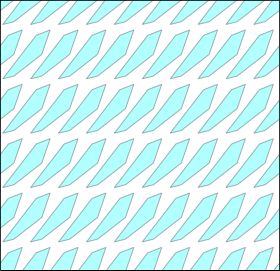
\includegraphics[width=.3\textwidth]{plavo_p1.png}
    \label{fig:plavop1}
    \caption{Група типа \textbf{p1}}
  \end{figure}



Кристалографску групу типа \textbf{p2} (Слика \ref{fig:plavop2}) генеришу централне централне симетрије у тачкама $A,B$ и $C$. Ради лакшег имплементирања, као генераторе ћемо посматрати једну рефлексију и две транслације тако што је $\mathcal{R}_B \circ \mathcal{R}_A = \mathcal{T}_{2\vec{AB}} $ и $\mathcal{R}_C \circ \mathcal{R}_A = \mathcal{T}_{2\vec{AC}} $, па је генератор те групе $\left\{ \mathcal{R}_A , \mathcal{T}_{2\vec{AB}}, \mathcal{T}_{2\vec{AC}} \right\} $.  Генеришемо га помоћу вектора тих транслација и координата тачке $A$. У матричном облику то је 

$$\left\{\begin{bmatrix}-1 & 0 & 2A_x\\ 0 & -1&2A_y \\ 0 & 0 & 1\end{bmatrix}, \begin{bmatrix}1 & 0 & u_x\\ 0 & 1&u_y \\ 0 & 0 & 1\end{bmatrix},  \begin{bmatrix}1 & 0 & v_x\\ 0 & 1&v_y \\ 0 & 0 & 1\end{bmatrix}\right\} $$

\begin{figure}[H]
\centering
    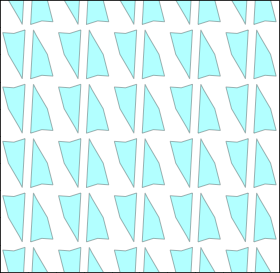
\includegraphics[width=.3\textwidth]{plavo_p2.png}
    \label{fig:plavop2}
    \caption{Група типа \textbf{p2}}
  \end{figure}



Кристалографску групу типа \textbf{pm}  (Слика \ref{fig:plavopm}) генеришу две рефлексије са паралелним осама $a$ и $b$ и транслација за вектор $u$, паралелан са тим осама. Нека су тачке $A$ и $B$ редом на правама $a$ и $b$ тако да је $AB \perp a$. Како су осе паралелне, важи да је $\mathcal{S}_b \circ \mathcal{S}_a = \mathcal{T}_{2\vec{AB}}$. За генератор групе можемо изабрати $\left\{ \mathcal{S}_a , \mathcal{T}_{2v}, \mathcal{T}_{u} \right\} $, где је  вектор $v = \vec{AB}$. Ако права $a$ пролази кроз координатни почетак, генератор у матричном облику је
$$\left\{\begin{bmatrix} \frac{{A_x}^2-{A_y}^2}{{A_x}^2+{A_y}^2} & \frac{2A_x A_y}{{A_x}^2+{A_y}^2} & 0\\ \frac{2A_x A_y}{{A_x}^2+{A_y}^2} & \frac{{A_y}^2-{A_x}^2}{{A_x}^2+{A_y}^2}&0 \\ 0 & 0 & 1\end{bmatrix} & ,& \begin{bmatrix}1 & 0 & 2v_x\\ 0 & 1&2v_y \\ 0 & 0 & 1\end{bmatrix}&,& \begin{bmatrix}1 & 0 & u_x\\ 0 & 1&u_y \\ 0 & 0 & 1\end{bmatrix}  \right\} $$


\begin{figure}[H]
\centering
    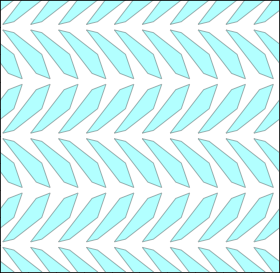
\includegraphics[width=.3\textwidth]{plavo_p3.png}
    \label{fig:plavopm}
    \caption{Група типа \textbf{pm}}
  \end{figure}



На сличан начин можемо конструисати генераторе за преосталих 14 типова кристалографских група.

\section{Ефективно конструисање коначног подскупа кристалографске групе}

С обзиром на то да кристалографска група садржи бесконачно изометрија, није могуће ефективно конструисати целу кристалографску групу. У пракси, конструишемо неки подскуп те групе да  бисмо представили део поплочавања.

Можемо користити различите критеријуме за одређивање коначног подскупа а један од њих је $$G' = \{\sigma \in G \;|\; d(X,\sigma(X)) < r\} $$ где је $G$ дата група, $X$ изабрана тачка равни, $r$ изабрана константа и $d$ функција растојања.

Нека је Г генератор групе $G$. Дефинишимо низ скупова изометрија $G_n$ тако да је $$G_0 = \{I\}$$
$$G_{n+1} = G_n \cup \{\sigma \circ \rho \;|\; \sigma \in G_n\; \wedge \; \rho \in \Gamma \cup \Gamma^{-1} \wedge \; d(X,(\sigma \circ \rho)(X)) < r \}. $$

С обзиром на то да је $G_0 \subset G'$ и да из услова $d(X,\sigma(X)) < r$ произилази 
$$G_n \subset G' \Rightarrow G_{n+1} \subset G'$$ индукцијом заклључујемо да је $$G_n \subset G'$$ за свако $n \in \mathbb{N_0}.$

Из дефиниције непосредно произилази да je $G_n \subset G_{n+1}$, што значи да постоји \\ $n_0\in \mathbb{N_0}$ тако да је $G_{n+1} = G_n$, за свако $n\geq n_0$. У супротном, $G'$ не би био коначан скуп. Овим смо описали поступак конструисања $G''= G_{n_0}$, који се може ефективно спровести. Приметимо да $G''$ не мора бити једнако $G'$, али у пракси можемо изабрати довољно велико $r$ тако да  изометрије из $G''$ одређују део поплочавања који приказујемо. 

У рачунарској имлементацији за дату кристалоргафску групу $G$ на почетку одређујемо $G''$ у форми скупа матрица, тако да после можемо ефикасно исцртавати поплочавања за различите облике плочица.





\chapter{Фундаментални домени и њихова конструкција}\label{dirihleova-fundamentalna-oblast} 

Да бисмо конструисали поплочавање, поред кристалографске групе потребно је да конструишемо и плочицу на коју примењујемо изометрије групе. Конструисаћемо плочицу која је фундаментални домен.

У овом поглављу ћемо описати конструкцију Дирихлеовог домена као и уопштења Дирихлеовог домена.
\section{Воронојев дијаграм}


Посматрајмо раван $\pi$ и две произвољне тачке $A$ и $B$ у њој. Поделимо је симетралом дужи $AB$ на две полуравни $\pi _A$ и $\pi _B$, тако да $A \in \pi _ A$ и $B \in \pi _B$. Јасно је да су све тачке на симетрали једнако удаљене од тачака $A$ и $B$, као и да је свакој тачки у $\pi _A$ ближа тачка $A$ него тачка $B$ и обрнуто. 
На тај начин смо све тачке равни $\pi$ поделили на два подскупа према томе којој од тачака $A$ и $B$ су ближе, а на рубу тих скупова (симетрала дужи $AB$) су тачке које су једнако удаљене од $A$ и $B$.

Уопштимо овај поступак за коначан број почетних тачака.

Означимо редом са $\pi _{XY}$ и $\pi _{YX}$ отворене полуравни којима симетрала дужи $XY$ дели раван $\pi$ на две полуравни тако да $X \in \pi _ {XY}$ и $Y \in \pi _{YX}$. 

Уколико на почетку имамо три тачке $A$, $B$ и $C$, тада је $\pi _{AB}$ скуп свих тачака у равни којима је тачка $A$ ближа него тачка $B$ и $\pi _{AC}$ скуп тачака којима је тачка $A$ ближа него тачка $C$, па је $\pi _{AB} \cap \pi _{AC}$ скуп тачака којима је тачка $A$ најближа тачка.

Применом овог поступка на  $n$ тачака, $A_1$, $A_2$, ... $A_n$ добијамо да је скуп тачака којима је $A_i$ најближа   $$\bigcap _{1\leq ј\leq н,\; ј\neq i} \pi_{A_i А_ј}.$$

Оваквку поделу равни на области према растојњу од датих тачака назива се \emph{Воронојевим дијаграмом} према руском матетичару \emph{Георгију Вороноју} (Слика 4.1).

\begin{figure}[H]
    \centering
    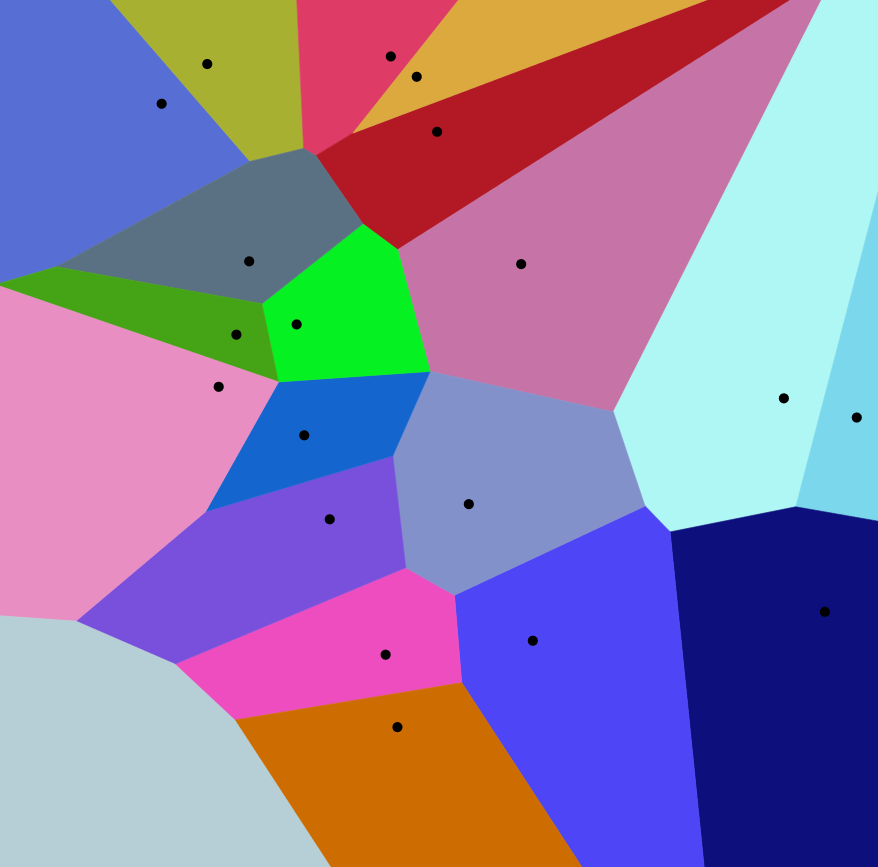
\includegraphics[width=.4\textwidth]{voronoiiii.png}
    \caption{Воронојев дијаграм}
    \label{fig:my_label}
\end{figure}

\begin{definition}%(voronijev dijagram)
За скуп тачака равни $S$, Воронојев дијаграм је подела равни на затворене дисјунктне области $V_S(A_i)$, које називамо Воронојевим  ћелијама, таква да
$$ (\forall X \in V_{S}(A))(\forall B \in S\setminus \{A\})\quad d(X,A)\leq d(X,B) $$
$$ \bigcup_{\forall A \in S} V_{S}(A) = \mathbb{E}^2 .$$

\end{definition}

Из претходног разматрања произилази
$$V_S(A) = \bigcap _{B \in S \setminus \{A\}} \pi_{AB}.$$ 

\section{Дирихлеов домен}

Воронојеви дијаграми су један метод конструисања фундаменталног домена кристалографске групе $G$ тако што је $S$ орбита неке тачке $X$. Тада је Воронојев дијаграм поплочавање равни под дејством $G$, а свака ћелија дијаграма је фундаментални домен. \\
Такав фундаментални домен назива се \emph{Дирихлеов домен}.

Са $O_G(X)$ означавамо орбиту тачке $X$, односно
$$O_G(X) = \{g(X)\:|\:g \in G\} .$$

\begin{definition}
За дату тачку $X$ и кристалографксу групу $G$ Дирихлеов домен означавамо са $D_G(X)$ и важи
$$D_G(X) = \{Y \in \mathbb{E}^2\:|\:(\:\forall g \in G \setminus \{I\})\:(d(Y,X)\leq d(Y,g(X))\:\}.$$
\end{definition}

\noindent  Докажимо да овако дефинисан Дирихлеов домен јесте фундаментални домен за кристалографксу групу $G$.
Дирихлеов домен можемо посматрати као ћелију Воронојевог дијаграма 
$$D_G(X)= V_{O_G(X)}(X).$$

\noindent Како важи $d(g(X), g(Y))= d(X,Y)$ то је  $D_G(g(X)) = g(D_G(X))$  .
Такође приметимо да $$Y \in  O_G(X) \implies O_G(Y) = O_G(X) $$
На основу претходног важи

$$\bigcup_{g\in G}g(D_G(X)) = \bigcup_{g\in G}D_G(g(X)) = \bigcup_{y \in O_G(X)}D_G(Y)
= \bigcup_{Y \in O_G(X)}V_{O_G(Y)}(Y) = \mathbb{E}^2.$$

\noindent Тиме смо доказали први услов из дефиниције фундаменталног домена, да његове слике прекривају целу раван.

\noindent Слично закључујемо да за $Y = g(X)$
$$g(D_G(X)) = D_G(Y) = V_{O_G(Y)}(Y)$$ што значи да су $D_G(X)$ i $D_G(Y)$ различите ћелије Воронојевог дијаграма, па им сед унутрашњости не секу. 

Тиме смо доказали и други услов из дефиниције фундаменталног домена, да се његове слике не преклапају. Дакле, доказали смо да је $D_G(X)$ фундаментални домен групе $G$.

На наредним примерима приказани су примери Дирихлеових домена за групу \textbf{p6} и произвољне тачке. 
Група \textbf{p6} је генерисана ротацијом за угао \(\frac{2\pi}{3}\) око једног
и \(\frac{\pi}{3}\) око друга два темена троугла са угловима \(\frac{2\pi}{3}\), \(\frac{\pi}{6}\) i \(\frac{\pi}{6}\).



  \begin{figure}[H]
  \begin{subfigure}[b]{0.32\textwidth}
    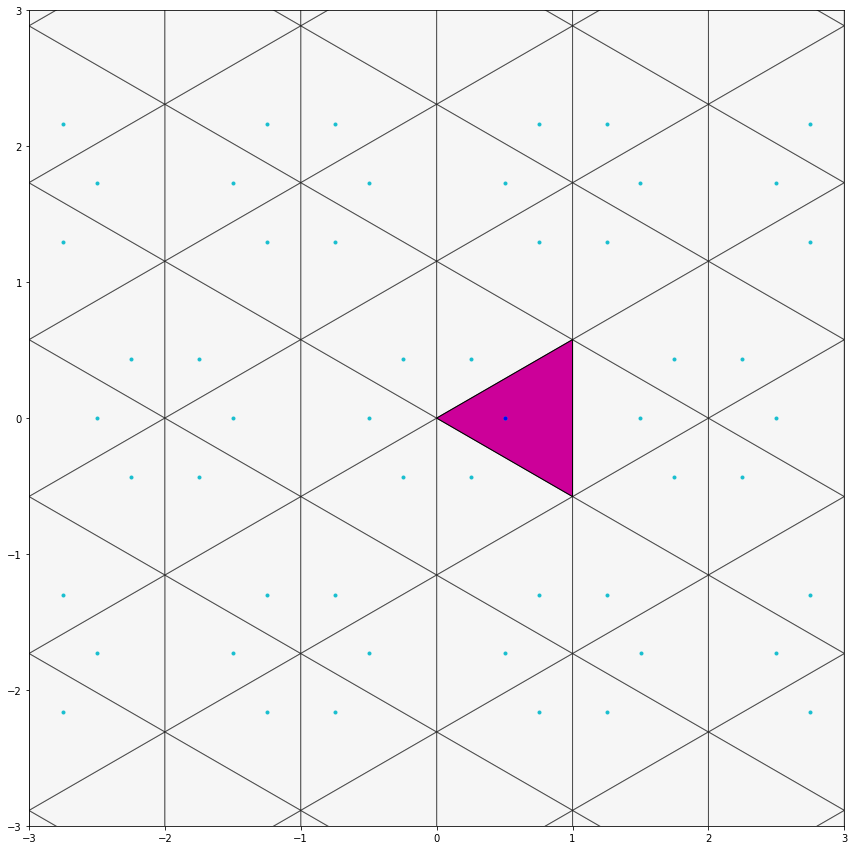
\includegraphics[width=.9\textwidth]{dirihleov1.png}
    \label{fig:f1}
  \end{subfigure}
  \begin{subfigure}[b]{0.32\textwidth}
    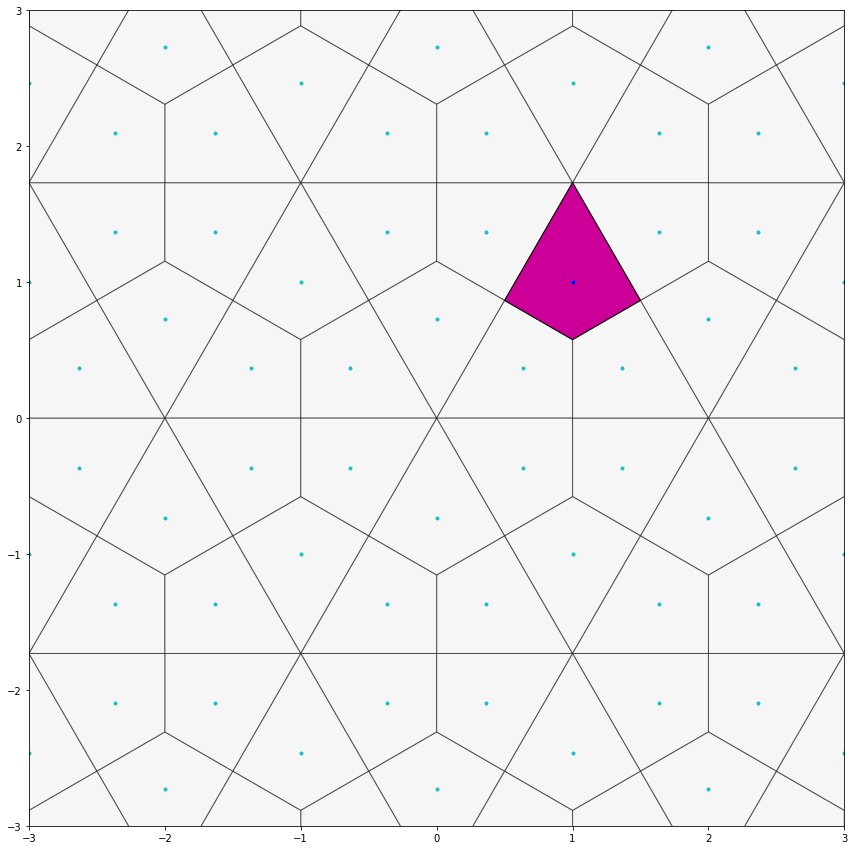
\includegraphics[width=.9\textwidth]{dirihleov2.png}
    \label{fig:f2}
  \end{subfigure}
  \begin{subfigure}[b]{0.32\textwidth}
    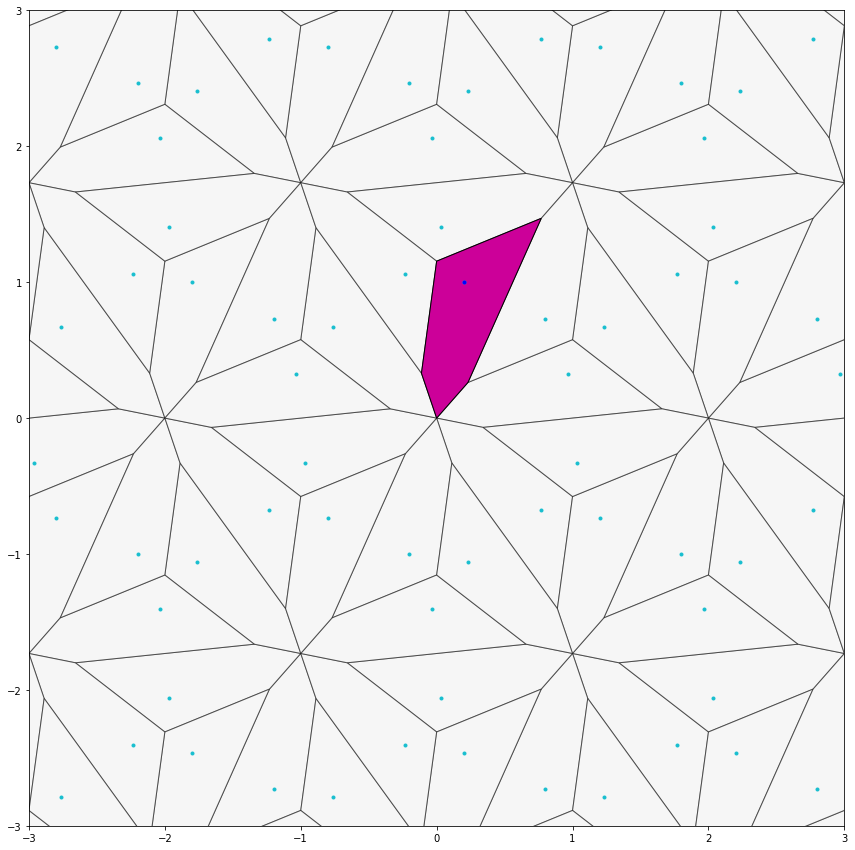
\includegraphics[width=.9\textwidth]{dirihleov3.png}
    \label{fig:f3}
  \end{subfigure}
\end{figure}


    \section{Уопштени Дирихлеов домен за више тачака}\label{konstrukcija-dirihleove-fundamentalne-oblasti}
    
Слично Дирихлеовом домену за једну тачку,  можемо посматрати домен генерисан двема тачкама. Тада нам је  $O_G(\{X,Y\})$ скуп тачака које се могу добити изометријама од једне од те две тачке. Посматрајмо Воронојев дијаграм над свим тачкама орбите $O_G(\{X,Y\})$.  Унија Воронојевих ћелија за тачку $X$ и за тачку $Y$ је фундаментални домен групе $G$, што је у општем случају исказано следећим тврђењем
\begin{tvrdjenje}
Нека је $S$ коначан скуп тачака равни на коју делује кристалографска група $G$, тада је 
$$D_G(S) = \{x \in \mathbb{E}^2\:|\:(\:\forall g \in G \setminus \{I\})\:(d(X,S)\leq d(X,g(S))\:\}$$

фундаментални домен групе $G$, где је $d(X,S) = \min_{Y \in S} d(X,Y)$ i va\v zi 
$$D_G(S) = \bigcup_{X \in S} V_{O_G(S)}(X) $$ 
\end{tvrdjenje}

%Doka\v zimo prvo drugi deo tvr\dj enja. 
%Posmatrajmu ta\v cku $Y$ takvu da $Y \in D_G(X)$. Tada je $(\:\forall X_1 \in O_G(S))\:(d(Y,X)\leq d(Y,X_1)$
%$$D_G(S) = \bigcup_{X \in S} D_G(X) $$

%nastavice se

\begin{samepage}
На примерима видимо уопштен Дирихлеов домен за две, три и четири произвољне тачке и групу \textbf{p6}.

\begin{figure}[H]
  \begin{subfigure}[b]{0.32\textwidth}
    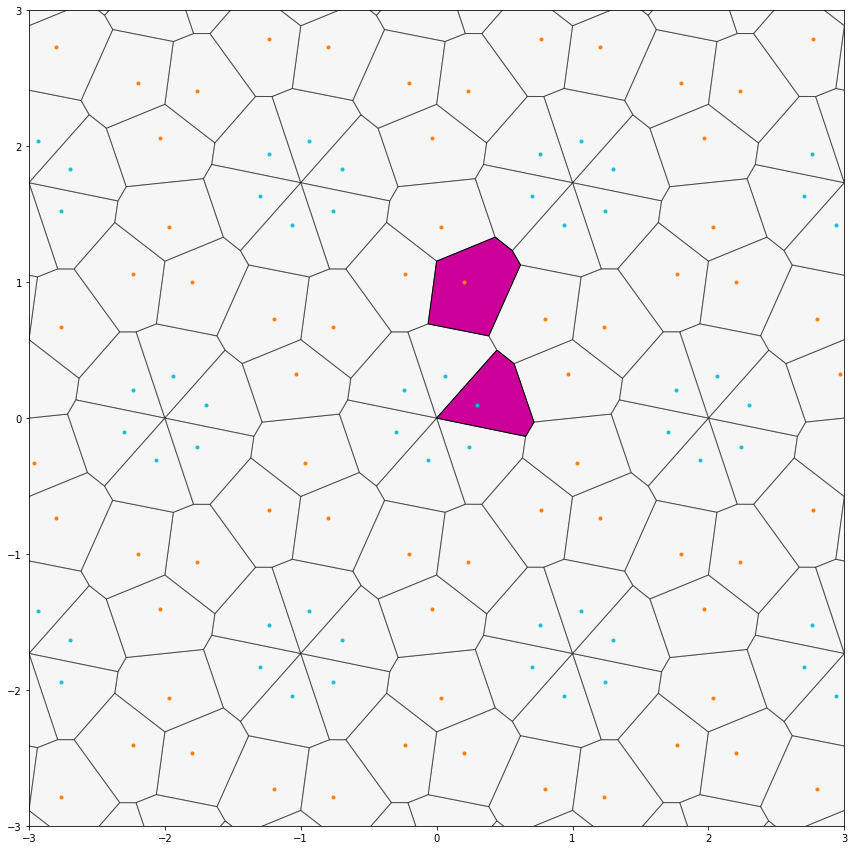
\includegraphics[width=.9\textwidth]{visetacaka1.png}
    \label{fig:f4}
  \end{subfigure}
  \begin{subfigure}[b]{0.32\textwidth}
    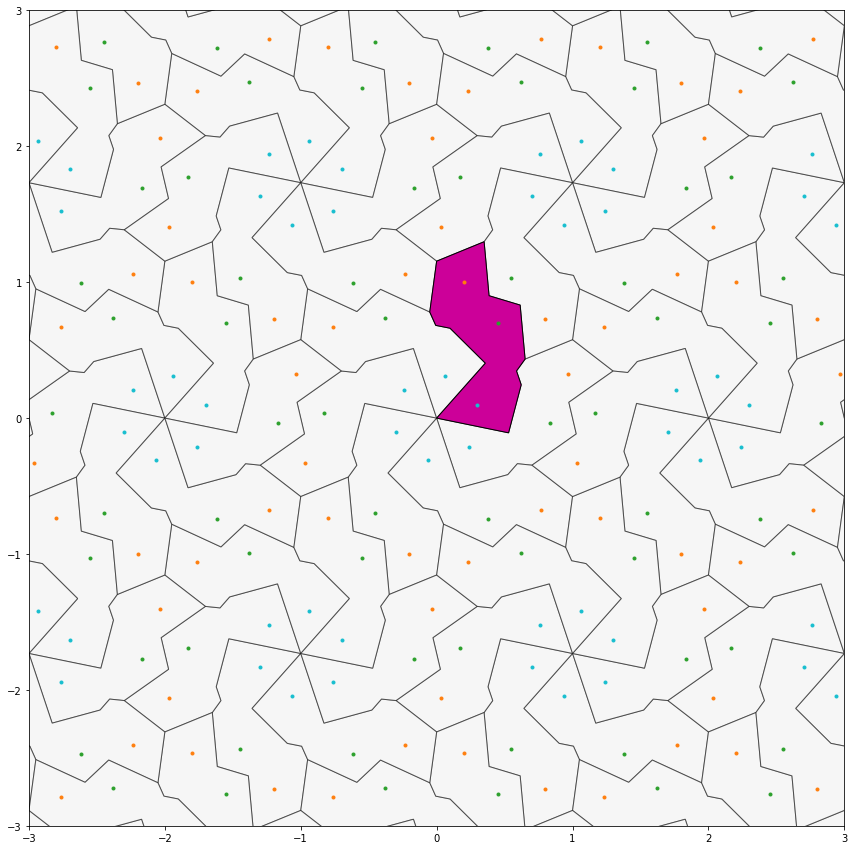
\includegraphics[width=.9\textwidth]{visetacaka2.png}
    \label{fig:f5}
  \end{subfigure}
  \begin{subfigure}[b]{0.32\textwidth}
    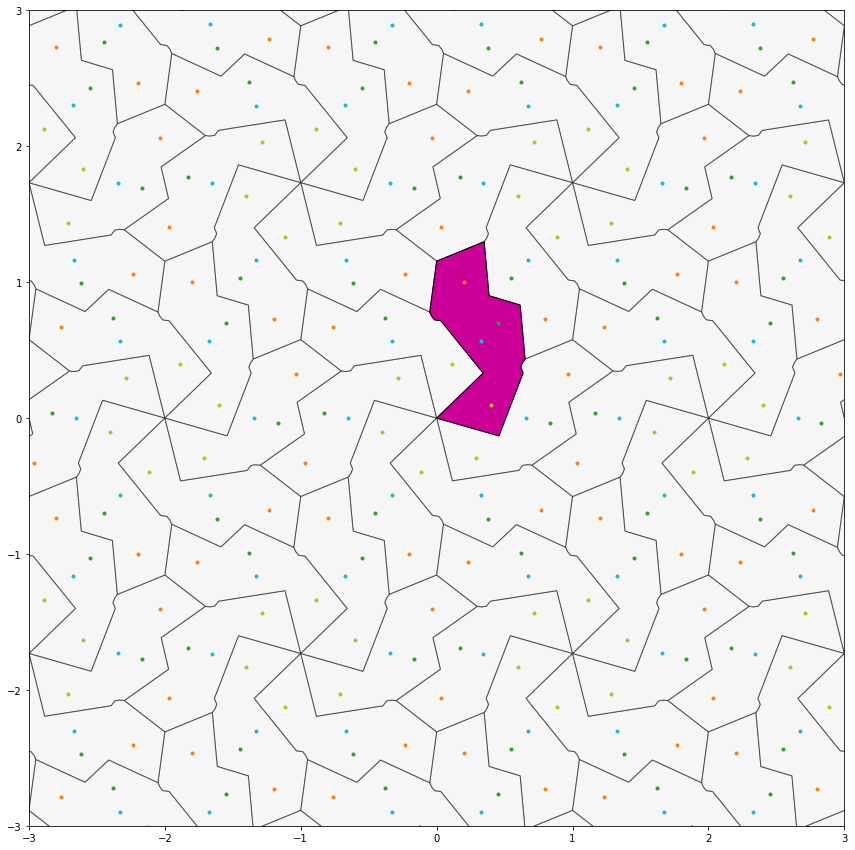
\includegraphics[width=.9\textwidth]{visetacaka3.png}
    \label{fig:f6}
  \end{subfigure}
\end{figure}
\end{samepage}

    \section{Уопштени Дирихлеов домен за полигон}\label{modifikacija-fundamentalne-oblasti-na-osnovu-podfundamentalne}
Дефиниција Дирихлеовог домена се може уопштити и када скуп $S$ није коначан, а конструкција Воронојевог дијаграма у том случају се може извести као гранична вредност када бирамо све већи број тачака.

Нека је дат полигон $P$ тако да се слике полигона у орбити не пресецају. 


Нека је $S_0$ скуп темена полигона $P$, а $S_n$ скуп у коме су поред темена полигона и по $n$ тачака са сваке од страница полигона на једнаким растојањима у оквиру странице.

На слици 7 је дат пример за $D_G(S_0)$.Он јесте фундаментални домен али приметимо да не обухвата цео полигон $P$.

На слици 8 је приказан $D_G(S_1)$, где су укључена и средишта страница и приметићујемо да тај фундаментални домен боље покрива почетни полигон. 


Уопштени Дирихлеов домен за полигон можемо да дефинишемо исто као и за коначан скуп
$$D_G(P) = \{X \in \mathbb{E}^2\:|\:(\:\forall g \in G \setminus \{I\})\:(d(X,P)\leq d(X,g(P))\:\}$$
при чему је $d(X,P) = \inf_{Y \in P} d(X,Y)$  и тада важи
$$ D_G(P) = \lim _{n\to \infty} D_G(S_n). $$


За практичне потребе треба узети довољно велико $n$. На слици 9 дат је пример за $D_G(S_{50})$

  \begin{figure}[H]
  \begin{subfigure}[b]{0.32\textwidth}
    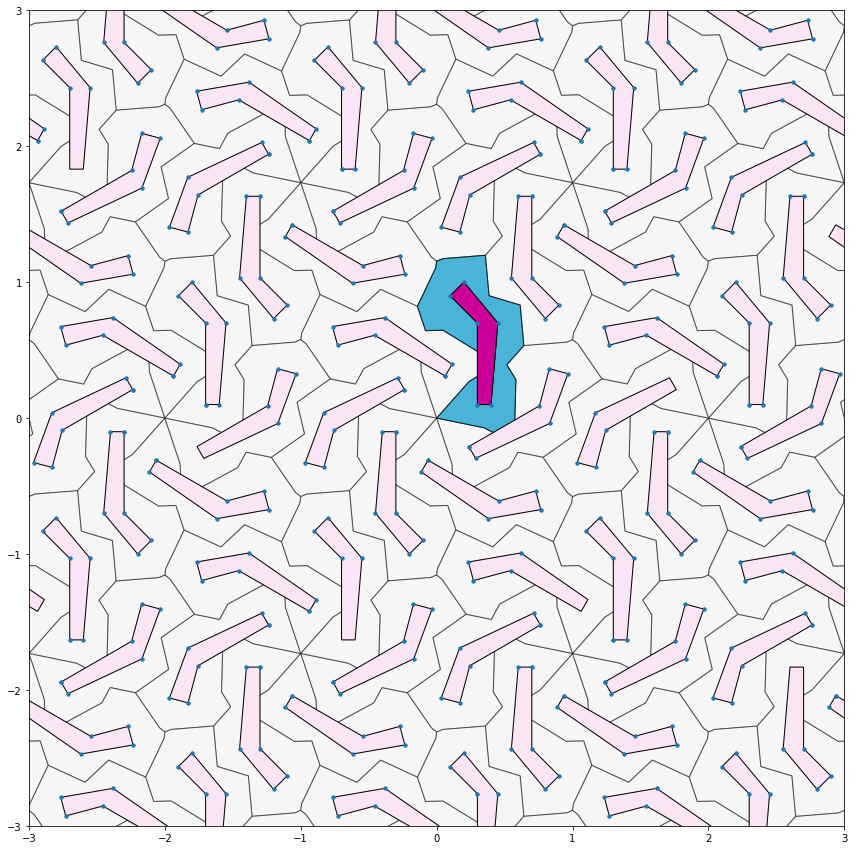
\includegraphics[width=.9\textwidth]{poligon1.png}
    \label{fig:f7}
  \end{subfigure}
  \begin{subfigure}[b]{0.32\textwidth}
    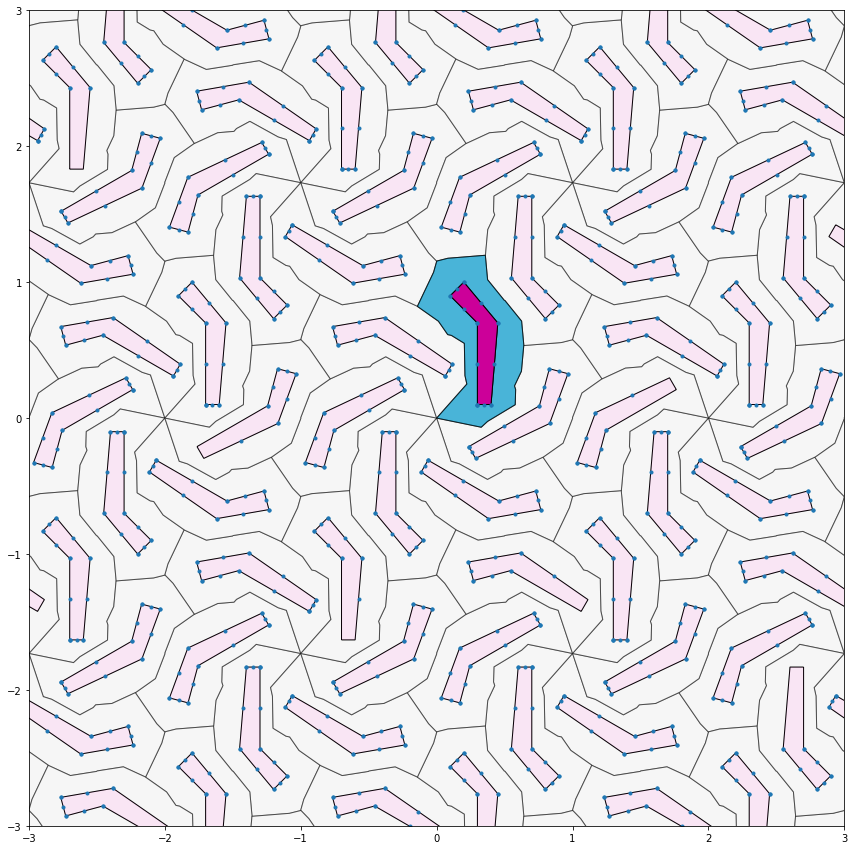
\includegraphics[width=.9\textwidth]{poligon2.png}
    \label{fig:f8}
  \end{subfigure}
  \begin{subfigure}[b]{0.32\textwidth}
    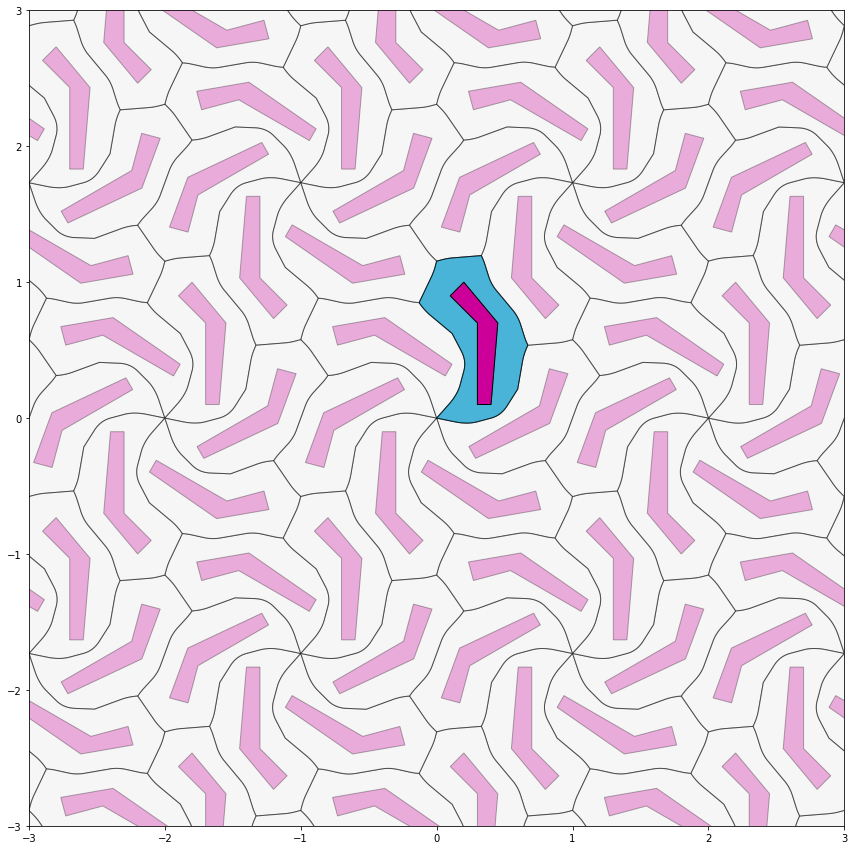
\includegraphics[width=.9\textwidth]{poligon3.png}
    \label{fig:f9}
  \end{subfigure}
\end{figure}

\begin{samepage}
 На следећим сликама су дати примери уопштених дирихлеових домена за исти полигон у разним кристалографским групама.
 \begin{figure}[H]

  \begin{subfigure}[b]{0.3\textwidth}
    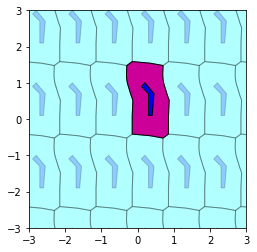
\includegraphics[width=\textwidth]{output_21_1.png}
    \label{fig:f20}
    \caption{G \textbf{p1}}
  \end{subfigure}
  \begin{subfigure}[b]{0.3\textwidth}
    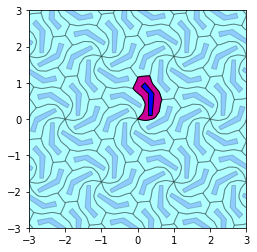
\includegraphics[width=\textwidth]{output_21_2.png}
    \label{fig:f21}
    \caption{grupa \textbf{p2}}
  \end{subfigure}
  \begin{subfigure}[b]{0.3\textwidth}
    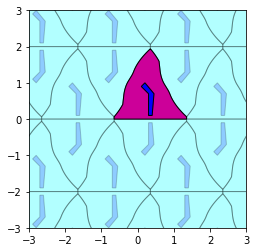
\includegraphics[width=\textwidth]{output_21_10.png}
    \label{fig:f24}
    \caption{grupa \textbf{pg}}
  \end{subfigure}

  \begin{subfigure}[b]{0.3\textwidth}
    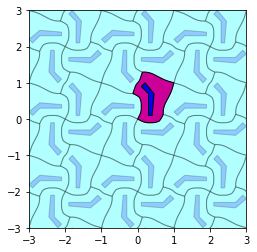
\includegraphics[width=\textwidth]{output_21_4.png}
    \label{fig:f23}
    \caption{grupa \textbf{p4}}
  \end{subfigure}
  \begin{subfigure}[b]{0.3\textwidth}
    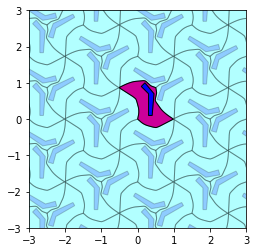
\includegraphics[width=\textwidth]{output_21_3.png}
    \label{fig:f22}
    \caption{grupa \textbf{p3}}
  
  \end{subfigure}
  \begin{subfigure}[b]{0.3\textwidth}
    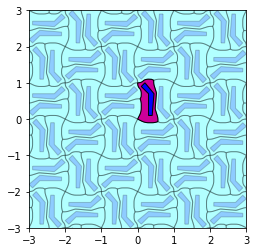
\includegraphics[width=\textwidth]{output_21_7.png}
    \label{fig:f25}
    \caption{grupa \textbf{cmm}}
  \end{subfigure}
\end{figure}
\end{samepage}

\quad \\ \qquad
    \chapter{Имплементација}\label{implementacija}

На основу претходно описаних метода конструкције кристалоградске групе и фундаменталних домена, имплементирана је рачунарска апликација која омогућава интерактивну конструктцију фундаменталног домена за изабрану кристалографску групу.
Апликација се може користити за дизајнирање занимљивих поплочавања.
Имплементира је рађена у програмском језику Пајтон.

На приказаним изгледима екрана (Слика \ref{slk_rad}) корисник додаје тачку по тачку кликом миша и на тај начин обликује фундаментални домен. За конструкцију фундаменталних домена поред изабраних тачака коришћене су додатне тачке између њих како би облик фундаменталног домена био мекши. 


\begin{figure}[h]

  \begin{subfigure}[b]{0.323\textwidth}
    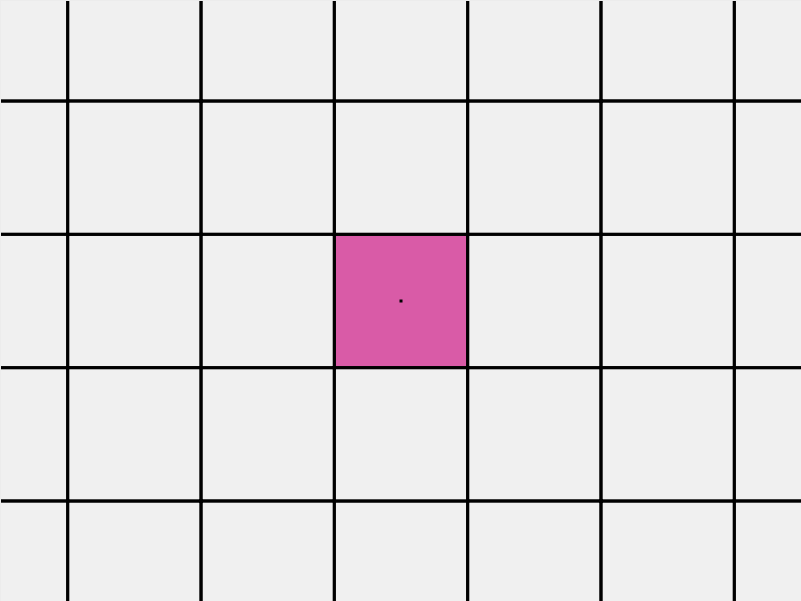
\includegraphics[width=0.9\textwidth]{s0.png}

  \end{subfigure}
  \begin{subfigure}[b]{0.323\textwidth}
    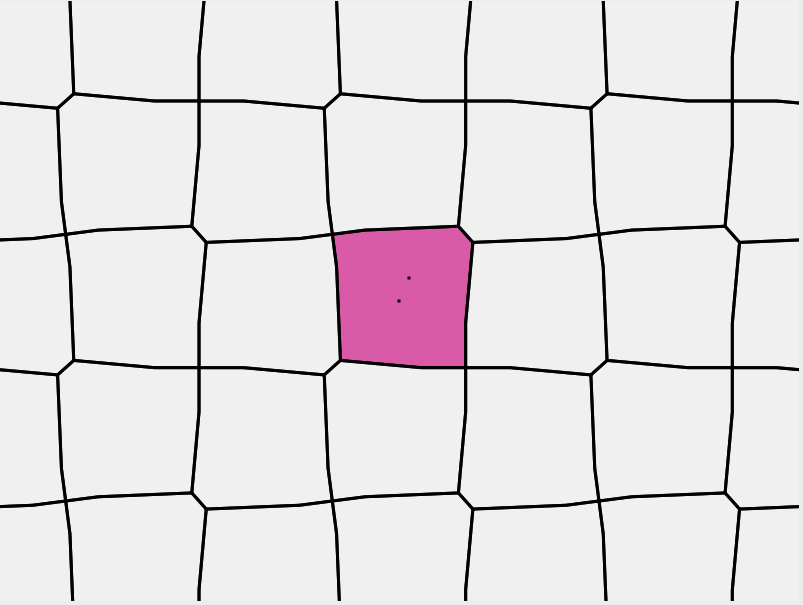
\includegraphics[width=0.9\textwidth]{s1.png}

  \end{subfigure}
  \begin{subfigure}[b]{0.323\textwidth}
    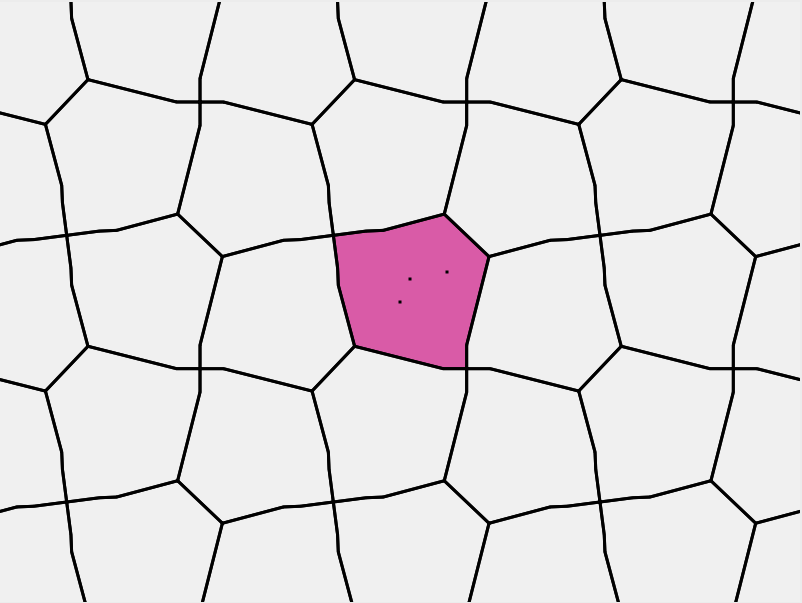
\includegraphics[width=0.9\textwidth]{s2.png}

  \end{subfigure}

\quad

%  \begin{subfigure}[b]{0.3\textwidth}
%    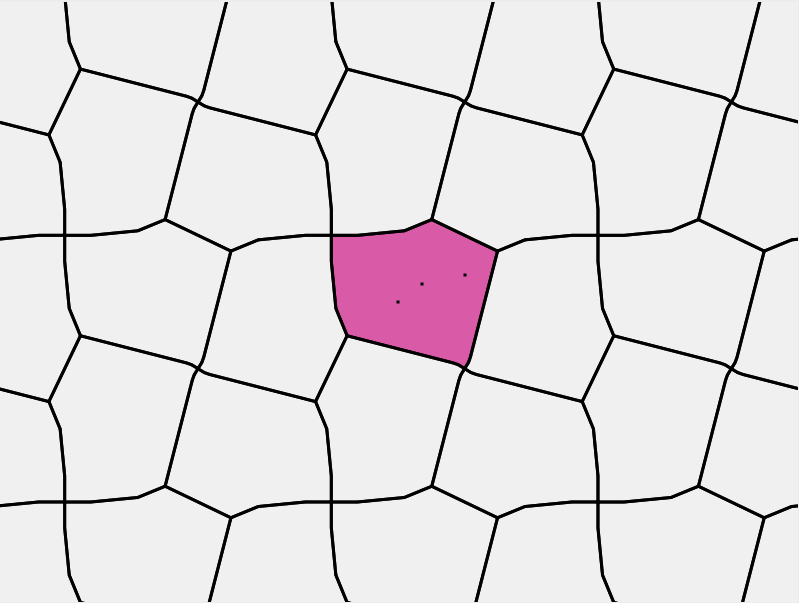
\includegraphics[width=.9\textwidth]{s4.png}

%  \end{subfigure}
  \begin{subfigure}[b]{0.5\textwidth}
    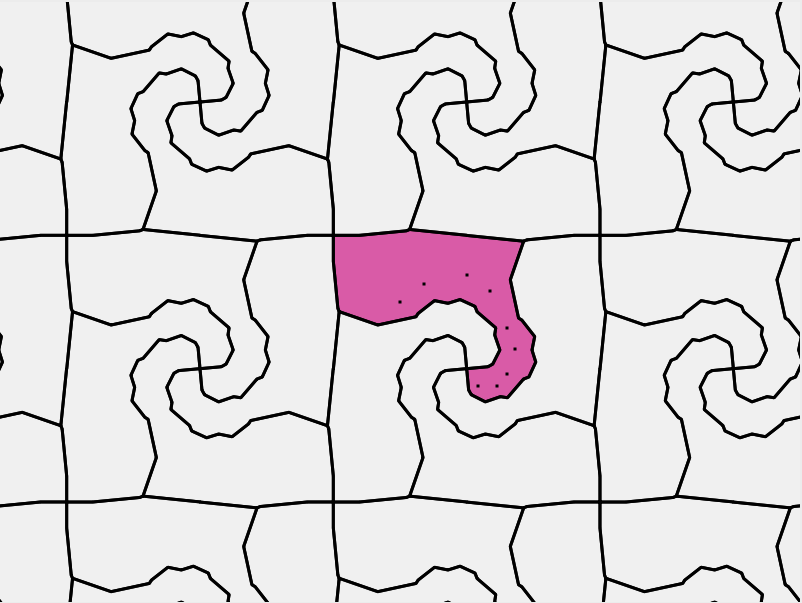
\includegraphics[width=.9\textwidth]{s5.png}

  
  \end{subfigure}
  \begin{subfigure}[b]{0.5\textwidth}
    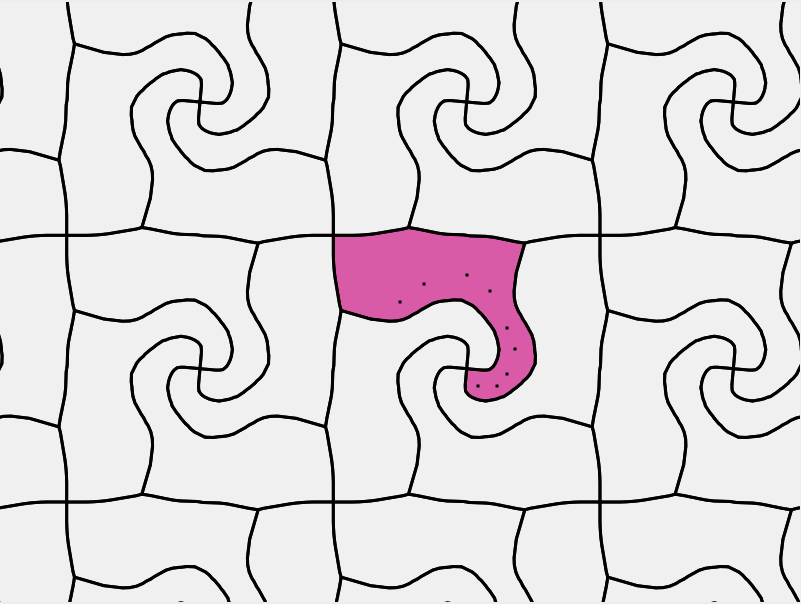
\includegraphics[width=.9\textwidth]{s6.png}

  \end{subfigure}
  \caption{Пример рада програма}
  \label{slk_rad}
\end{figure}

\chapter {Закључак}
У раду су обрађени појмови у вези са поплочавањем и кристалографским групама. Описан је метод конструкције фундаменталних домена кристалографских група еуклидске равни, као и метод конструкције саме кристалографске групе. Математички је описана метода конструкције фундаменталних домена заснована на уопштењу Дирихлеовог домена и имплементирана је рачунарска апликација која ефективно конструише фундаменталне домене коришћењем те методе. Корисник апликације кликом миша уцртава тачке. На основу задатих тачака програм констурише фундаментални домен коме припрадају све тачке равни које су ближе некој од задатих тачака него некој од њихових слика у изометријама из кристалографске групе и у реалном времену се исцртава добијено поплочавање. Апликација има опцију да изабрани скуп тачака посматра као темена изломљене линије, на основу које се конструише фундаментални домен као скуп тачака равни којима је та изломљена линија ближа него било која њена слика. 




\renewcommand\bibname{Литература}
\begin{thebibliography}{}

\bibitem{1}  Carne, T. K.  "Geometry and groups." Lecture notes, Cambridge University (2006). 
\bibitem{6}
Grünbaum B, Shephard GC."Tilings and patterns." Freeman (1987).
 \bibitem{4}  Kaplan, Craig S. "Introductory tiling theory for computer graphics."{} Synthesis Lectures on Computer Graphics and Animation 4.1 (2009): 1-113. 
 \bibitem{6}  Kilgore, J. "Fundamental Domains of Discrete Groups Acting on Euclidean Space." (2012). 
 \bibitem{2} Lučić, Z., and Molnár, E. "{}Combinatorial classification of fundamental domains of finite area for planar discontinuous isometry groups." Archiv der Mathematik 54.5 (1990): 511-520.
\bibitem{1} Molnár, E. "Nice tiling, nice geometry." Teaching Mathematics and Computer Science, Debrecen (2012): 269-280.


\bibitem{5} 
  Schattschneider, D. "The plane symmetry groups: their recognition
  and notation." \emph{The American Mathematical Monthly} 85.6 (1978):
  439-450.



\end{thebibliography}





	

\end{document}
